%%%%%%%%%%%%%%%%%%%%%%%%%%%%%%%%%%%%%%%%%
% Short Sectioned Assignment LaTeX Template Version 1.0 (5/5/12)
% This template has been downloaded from: http://www.LaTeXTemplates.com
% Original author:  Frits Wenneker (http://www.howtotex.com)
% License: CC BY-NC-SA 3.0 (http://creativecommons.org/licenses/by-nc-sa/3.0/)
%%%%%%%%%%%%%%%%%%%%%%%%%%%%%%%%%%%%%%%%%

%----------------------------------------------------------------------------------------
%	PACKAGES AND OTHER DOCUMENT CONFIGURATIONS
%----------------------------------------------------------------------------------------

\documentclass[paper=a4, fontsize=11pt]{scrartcl} % A4 paper and 11pt font size

% ---- Entrada y salida de texto -----

\usepackage[T1]{fontenc} % Use 8-bit encoding that has 256 glyphs
\usepackage[utf8]{inputenc}

% ---- Idioma --------

\usepackage[spanish, es-tabla]{babel} % Selecciona el español para palabras introducidas automáticamente, p.ej. "septiembre" en la fecha y especifica que se use la palabra Tabla en vez de Cuadro

% ---- Otros paquetes ----

\usepackage{amsmath,amsfonts,amsthm} % Math packages
\usepackage{graphics,graphicx, floatrow} %para incluir imágenes y notas en las imágenes
\usepackage{graphics,graphicx, float} %para incluir imágenes y colocarlas
\usepackage{hyperref} % url in references
\usepackage{listings}
\usepackage{color}
\definecolor{grey}{gray}{0.9}

% Para hacer tablas comlejas
\usepackage{multirow}
\usepackage{threeparttable}

\usepackage{fancyhdr} % Custom headers and footers
\pagestyle{fancyplain} % Makes all pages in the document conform to the custom headers and footers
\fancyhead{} % No page header - if you want one, create it in the same way as the footers below
\fancyfoot[L]{} % Empty left footer
\fancyfoot[C]{} % Empty center footer
\fancyfoot[R]{\thepage} % Page numbering for right footer
\renewcommand{\headrulewidth}{0pt} % Remove header underlines
\renewcommand{\footrulewidth}{0pt} % Remove footer underlines
\setlength{\headheight}{13.6pt} % Customize the height of the header

\numberwithin{equation}{section} % Number equations within sections (i.e. 1.1, 1.2, 2.1, 2.2 instead of 1, 2, 3, 4)
\numberwithin{figure}{section} % Number figures within sections (i.e. 1.1, 1.2, 2.1, 2.2 instead of 1, 2, 3, 4)
\numberwithin{table}{section} % Number tables within sections (i.e. 1.1, 1.2, 2.1, 2.2 instead of 1, 2, 3, 4)

\setlength\parindent{0pt} % Removes all indentation from paragraphs - comment this line for an assignment with lots of text

\newcommand{\horrule}[1]{\rule{\linewidth}{#1}} % Create horizontal rule command with 1 argument of height

\usepackage{textcomp}
\usepackage{hyperref}

%----------------------------------------------------------------------------------------
%	DATOS
%----------------------------------------------------------------------------------------

\newcommand{\myName}{Francisco Javier Bolívar Lupiáñez}
\newcommand{\myDegree}{Máster en Ingeniería Informática}
\newcommand{\myFaculty}{E. T. S. de Ingenierías Informática y de Telecomunicación}
\newcommand{\myDepartment}{Ciencias de la Computación e Inteligencia Artificial}
\newcommand{\myUniversity}{\protect{Universidad de Granada}}
\newcommand{\myLocation}{Granada}
\newcommand{\myTime}{\today}
\newcommand{\myTitle}{Práctica 1}
\newcommand{\mySubtitle}{Competición en Kaggle sobre Clasificación Binaria}
\newcommand{\mySubject}{Sistemas Inteligentes para la Gestión de la Empresa}
\newcommand{\myYear}{2016-2017}

%----------------------------------------------------------------------------------------
%	PORTADA
%----------------------------------------------------------------------------------------


\title{	
	\normalfont \normalsize 
	\textsc{\textbf{\mySubject \space (\myYear)} \\ \myDepartment} \\[20pt] % Your university, school and/or department name(s)
	\textsc{\myDegree \\[10pt] \myFaculty \\ \myUniversity} \\[25pt]
	\horrule{0.5pt} \\[0.4cm] % Thin top horizontal rule
	\huge \myTitle: \mySubtitle \\ % The assignment title
	\horrule{2pt} \\[0.5cm] % Thick bottom horizontal rule
	\normalfont \normalsize
}

\author{
	\myName \\ 
	\small Kaggle: \texttt{fblupi} \\
	\small Posición: 416, Puntuación: 0.81340
}

\date{\myTime} % Incluye la fecha actual
%----------------------------------------------------------------------------------------
%	INDICE
%----------------------------------------------------------------------------------------

\begin{document}
	
\definecolor{light-gray}{gray}{0.95}
	
\lstset {
	basicstyle=\scriptsize,
	frame=single,
	backgroundcolor=\color{grey}
}

\lstdefinestyle{R}{
	frame=single,
	numbers=left,
	language=R,
	basicstyle=\tiny\ttfamily,
	keywordstyle=\bfseries,
	commentstyle=\itshape,
	identifierstyle=\bfseries,
}
	
\setcounter{page}{0}

\maketitle % Muestra el Título
\thispagestyle{empty}

\newpage %inserta un salto de página

\tableofcontents % para generar el índice de contenidos

%\listoftables
%\listoffigures

\newpage

%----------------------------------------------------------------------------------------
%	DOCUMENTO
%----------------------------------------------------------------------------------------

\section{Exploración de datos}
\label{sec:exploracion-datos}

La primera fase que hay que realizar ante cualquier problema de este tipo es la exploración de datos para poner los cimientos sobre los que realizar el posterior proceso de análisis.
\\ \\
Los datos con los que contamos en el \textit{dataset} son \cite{KaggleTitanicData}:

\begin{itemize}
	\item \texttt{PassengerId}: Id único, no va a ser de utilidad
	\item \texttt{PClass}: Clase en la que viajaba
	\item \texttt{Name}: Nombre y título
	\item \texttt{Sex}: Sexo
	\item \texttt{Age}: Edad
	\item \texttt{SibSp}: Número de hermanos y/o cónyuges
	\item \texttt{Parch}: Número de padres y/o hijos
	\item \texttt{Ticket}: Id del billete
	\item \texttt{Fare}: Tarifa del viaje
	\item \texttt{Cabin}: Cabina donde se alojó
	\item \texttt{Embarked}: Dónde embarcó
\end{itemize}

De aquí podemos concluir que ni \texttt{PassengerId}, ni \texttt{Ticket} nos van a ser útiles pues son únicos. \texttt{Name} podría tener el mismo problema, pero se podría extraer el título para utilizarlo como información que puede resultar útil.
\\ \\
También hay otras variables como \texttt{Cabin} que son poco útiles pues tiene la mayoría de los valores perdidos.

\subsection{La importancia del sexo, la edad y la clase}

Se sabe que el protocolo por aquel entonces era el de mujeres y niños primero por lo que vamos a ver si de verdad se cumplió y nos puede ayudar a predecir quién murió y quién no \cite{TrevorStephensTutorial}.
\\ \\
En primer lugar, vamos a ver el porcentaje de supervivientes:

\begin{lstlisting}[style=R]
prop.table(table(train$Survived))
\end{lstlisting}

\begin{table}[H]
	\centering
	\caption{Porcentaje de supervivientes}
	\label{tab:die-survive}
	\begin{tabular}{|ll|}
		\hline
		Die       & Survive   \\ \hline
		0.6161616 & 0.3838384 \\ \hline
	\end{tabular}
\end{table}

de sexo:

\begin{lstlisting}[style=R]
prop.table(table(train$Sex))
\end{lstlisting}

\begin{table}[H]
	\centering
	\caption{Porcentaje de sexo}
	\label{tab:male-female}
	\begin{tabular}{|ll|}
		\hline
		Male     & Female   \\ \hline
		0.647587 & 0.352413 \\ \hline
	\end{tabular}
\end{table}

y de adultos (considerándose a partir de los 18 años):

\begin{lstlisting}[style=R]
train$Child <- 0
train$Child[train$Age < 18] <- 1
prop.table(table(train$Child))
\end{lstlisting}


\begin{table}[H]
	\centering
	\caption{Porcentaje de edad}
	\label{tab:child-adult}
	\begin{tabular}{|ll|}
		\hline
		Child     & Adult     \\ \hline
		0.1268238 & 0.8731762 \\ \hline
	\end{tabular}
\end{table}

Combinando edad y sexo tenemos el siguiente resultado:

\begin{lstlisting}[style=R]
aggregate(Survived ~ Child + Sex, data=train, FUN=function(x) {sum(x)/length(x)})
\end{lstlisting}

\begin{table}[H]
	\centering
	\caption{Supervivencia según edad y sexo}
	\label{tab:age-sex}
	\begin{tabular}{|ll|l|}
		\hline
		Age   & Sex    & Survived  \\ \hline
		Adult & Female & 0.7528958 \\
		Child & Female & 0.6909091 \\
		Adult & Male   & 0.1657033 \\
		Child & Male   & 0.3965517 \\ \hline
	\end{tabular}
\end{table}

con el que podríamos hacer un primer envío dando por supervivientes a todas las mujeres. Solo con eso se tendría una puntuación de 0.76555.
\\ \\
No obstante, podemos intentar afinar más pues vemos que los hombres que son niños casi llega al 50\% de posibilidades de supervivencia. Agregando otros datos importantes como la clase y la tarifa del viaje obtenemos:

\begin{lstlisting}[style=R]
train$Fare2 <- '30+'
train$Fare2[train$Fare < 30 & train$Fare >= 20] <- '20-30'
train$Fare2[train$Fare < 20 & train$Fare >= 10] <- '10-20'
train$Fare2[train$Fare < 10] <- '<10'
aggregate(Survived ~ Child + Fare2 + Pclass + Sex, data=train, FUN=function(x) {sum(x)/length(x)})
\end{lstlisting}

\begin{table}[H]
	\centering
	\caption{Supervivencia según edad, sexo, clase y tarifa}
	\label{tab:age-sex-fare-pclass}
	\begin{tabular}{|llll|l|}
		\hline
		Age   & Fare        & Pclass & Sex    & Survived   \\ \hline
		Adult & 20-30       & 1      & Female & 0.83333333 \\
		Adult & 30+         & 1      & Female & 0.98750000 \\
		Child & 30+         & 1      & Female & 0.87500000 \\
		Adult & 10-20       & 2      & Female & 0.90625000 \\
		Child & 10-20       & 2      & Female & 1.00000000 \\
		Adult & 20-30       & 2      & Female & 0.88000000 \\
		Child & 20-30       & 2      & Female & 1.00000000 \\
		Adult & 30+         & 2      & Female & 1.00000000 \\
		Child & 30+         & 2      & Female & 1.00000000 \\
		Adult & \textless10 & 3      & Female & 0.56140351 \\
		Child & \textless10 & 3      & Female & 0.85714286 \\
		Adult & 10-20       & 3      & Female & 0.50000000 \\
		Child & 10-20       & 3      & Female & 0.73333333 \\
		Adult & 20-30       & 3      & Female & 0.40000000 \\
		Child & 20-30       & 3      & Female & 0.16666667 \\
		Adult & 30+         & 3      & Female & 0.11111111 \\
		Child & 30+         & 3      & Female & 0.14285714 \\
		Adult & \textless10 & 1      & Male   & 0.00000000 \\
		Adult & 20-30       & 1      & Male   & 0.40000000 \\
		Adult & 30+         & 1      & Male   & 0.35365854 \\
		Child & 30+         & 1      & Male   & 1.00000000 \\
		Adult & \textless10 & 2      & Male   & 0.00000000 \\
		Adult & 10-20       & 2      & Male   & 0.11864407 \\
		Child & 10-20       & 2      & Male   & 0.75000000 \\
		Adult & 20-30       & 2      & Male   & 0.04761905 \\
		Child & 20-30       & 2      & Male   & 0.75000000 \\
		Adult & 30+         & 2      & Male   & 0.00000000 \\
		Child & 30+         & 2      & Male   & 1.00000000 \\
		Adult & \textless10 & 3      & Male   & 0.10931174 \\
		Child & \textless10 & 3      & Male   & 0.15384615 \\
		Adult & 10-20       & 3      & Male   & 0.12903226 \\
		Child & 10-20       & 3      & Male   & 0.71428571 \\
		Adult & 20-30       & 3      & Male   & 0.07142857 \\
		Child & 20-30       & 3      & Male   & 0.20000000 \\
		Adult & 30+         & 3      & Male   & 0.41666667 \\
		Child & 30+         & 3      & Male   & 0.07692308 \\ \hline
	\end{tabular}
\end{table}

donde podríamos afinar diciendo que si las mujeres son de la clase 3 y su tarifa es mayor a 20 murieron y los niños con tarifa mayor a 30 de clase 1 o 2 sobrevivieron. Con este pequeño árbol de decisión hecho manualmente explorando los datos obtenemos una puntuación mejor que la anterior de un total de 0.77990.

\section{Preprocesamiento de datos}
\label{sec:preprocesamiento}

En esta sección trataremos valores perdidos así como extraer nuevo conocimiento de distintas variables \cite{TrevorStephensTutorial}.

\subsection{Nombres y familias}

Como se comentó en la Sección \ref{sec:exploracion-datos}, los nombres podrían parecer únicos, pero se puede extraer información para clasificarlos por títulos y familias pues títulos más importantes podrían haber tenido prioridad para salvarse y las familias, al ir lo más probable juntas, tendrían posibilidad de sobrevivir o morir todos.
\\ \\
Esto se ha hecho tanto con los \textit{dataset} de \textit{train} como de \textit{test}:

\begin{lstlisting}[style=R]
combi <- rbind(train, test)
\end{lstlisting}

\subsubsection{Títulos}

En primer lugar vamos a extraer el título de cada una de las entradas y agregarlo como un atributo más:

\begin{lstlisting}[style=R]
combi$Name <- as.character(combi$Name)
combi$Title <- sapply(combi$Name, FUN=function(x) {strsplit(x, split='[,.]')[[1]][2]})
combi$Title <- sub(' ', '', combi$Title)
\end{lstlisting}

Con esto obtenemos:

\begin{itemize}
	\item \textit{Capt}: 1
	\item \textit{Col}: 4
	\item \textit{Don}: 1
	\item \textit{Dona}: 1
	\item \textit{Dr}: 8
	\item \textit{Jonkheer}: 1
	\item \textit{Lady}: 1
	\item \textit{Major}: 2
	\item \textit{Master}: 61
	\item \textit{Miss}: 260
	\item \textit{Mlle}: 2
	\item \textit{Mme}: 1
	\item \textit{Mr}: 757
	\item \textit{Mrs}: 197
	\item \textit{Ms}: 2
	\item \textit{Rev}: 8
	\item \textit{Sir}: 1
	\item \textit{the Countess}: 1
\end{itemize}

Agregando los grupos pequeños que significan los mismo:

\begin{lstlisting}[style=R]
combi$Title[combi$Title %in% c('Mme', 'Mlle')] <- 'Mlle'
combi$Title[combi$Title %in% c('Capt', 'Don', 'Major', 'Sir')] <- 'Sir'
combi$Title[combi$Title %in% c('Dona', 'Lady', 'the Countess', 'Jonkheer')] <- 'Lady'
combi$Title <- factor(combi$Title)
\end{lstlisting}

obtenemos:

\begin{itemize}
	\item \textit{Col}: 4
	\item \textit{Dr}: 8
	\item \textit{Lady}: 4
	\item \textit{Master}: 61
	\item \textit{Miss}: 260
	\item \textit{Mlle}: 3
	\item \textit{Mr}: 757
	\item \textit{Mrs}: 197
	\item \textit{Ms}: 2
	\item \textit{Rev}: 8
	\item \textit{Sir}: 5
\end{itemize}

\subsubsection{Familias}

Las familias grandes podrían tener más posibilidad de morir buscando a cada uno de los miembros para salvarse todos.
\\ \\
Lo primero que hay que hacer es combinar los campos \texttt{SibSp} y \texttt{Parch} que como vimos en la Sección \ref{sec:exploracion-datos} eran los que determinaban hermanos y/o cónyuges y padres y/o hijos:

\begin{lstlisting}[style=R]
combi$FamilySize <- combi$SibSp + combi$Parch + 1
\end{lstlisting}

Ahora extraeremos el apellido:

\begin{lstlisting}[style=R]
combi$Surname <- sapply(combi$Name, FUN=function(x) {strsplit(x, split='[,.]')[[1]][1]})
\end{lstlisting}

Ahora agregaremos ambos valores y daremos valor \textit{Small} a los que tienen 3 familiares o menos:

\begin{lstlisting}[style=R]
combi$FamilyID <- paste(as.character(combi$FamilySize), combi$Surname, sep="")
combi$FamilyID[combi$FamilySize <= 2] <- 'Small'
\end{lstlisting}

No obstante vemos que a veces no coincide el id con el número de miembros en esto. Esto puede ser porque haya familiares con distinto id por no estar casados o no haber cambiado el apellido de soltería. Para lidiar con esto se les dará valor \textit{Small}:

\begin{lstlisting}[style=R]
famIDs <- data.frame(table(combi$FamilyID))
famIDs <- famIDs[famIDs$Freq <= 2,]
combi$FamilyID[combi$FamilyID %in% famIDs$Var1] <- 'Small'
combi$FamilyID <- factor(combi$FamilyID)
\end{lstlisting}

\subsection{Edad}

El campo de edad tiene muchísimos valores perdidos (263) entre los datos de \textit{train} y de \textit{test}.

\begin{lstlisting}[style=R]
summary(combi$Age)
\end{lstlisting}

Para resolver esto, se va a realizar una predicción del valor de estas variables usando el árbol de decisión de la librería \texttt{rpart} con el método \texttt{anova} pues queremos predecir una variable contínua y no categórica.

\begin{lstlisting}[style=R]
Agefit <- rpart(Age ~ Pclass + Sex + SibSp + Parch + Fare + Embarked + Title + FamilySize,
                data=combi[!is.na(combi$Age),], 
                method="anova")
combi$Age[is.na(combi$Age)] <- predict(Agefit, combi[is.na(combi$Age),])
\end{lstlisting}

\subsection{Embarque}

El embarque tiene dos valores perdidos:

\begin{lstlisting}[style=R]
summary(combi$Embarked)
\end{lstlisting}

Como la mayoría salió desde Southampton, vamos a darle este valor:

\begin{lstlisting}[style=R]
which(combi$Embarked == '') # 62 830
combi$Embarked[c(62,830)] = "S"
combi$Embarked <- factor(combi$Embarked)
\end{lstlisting}

\subsection{Tarifa}

La tarifa tiene un valor perdido:

\begin{lstlisting}[style=R]
summary(combi$Fare)
\end{lstlisting}

Por lo que le daremos la mediana:

\begin{lstlisting}[style=R]
which(is.na(combi$Fare)) # 1044
combi$Fare[1044] <- median(combi$Fare, na.rm=TRUE)
\end{lstlisting}

\section{Técnicas de clasificación}

A continuación pasaremos a utilizar distintas técnicas de clasificación para ver con cuál obtenemos mejor resultado \cite{TrevorStephensTutorial}.

\subsection{\textit{Decision Tree}}

\subsubsection{Sin procesamiento}

En primer lugar se probó sin antes preprocesar como se ha descrito en la sección \ref{sec:preprocesamiento}.

\begin{lstlisting}[style=R]
fit <- rpart(Survived ~ Pclass + Sex + Age + SibSp + Parch + Fare + Embarked, data=train, method="class")
\end{lstlisting}

Obteniendo el siguiente árbol:

\begin{figure}[H]
	\centering
	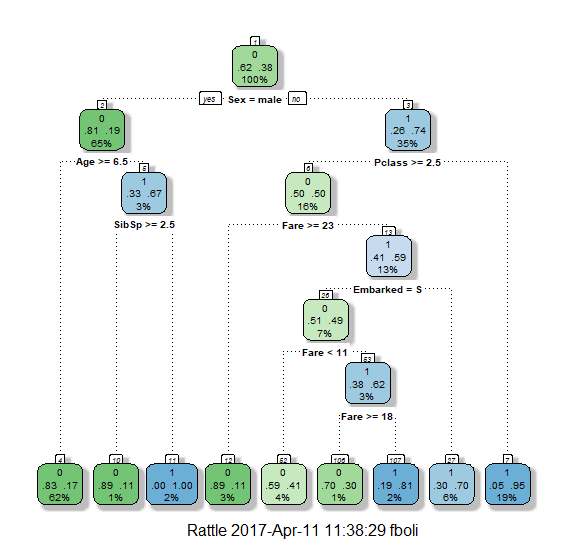
\includegraphics[width=14cm]{img/first-decision-tree}
	\caption{Primer árbol de decisión sin preprocesamiento}
	\label{fig:first-decision-tree}
\end{figure}

Con el que obtuvimos una puntuación de 0.78469.
\\ \\
También probamos el mismo pero haciendo que éste llegue hasta el final:

\begin{lstlisting}[style=R]
fit <- rpart(Survived ~ Pclass + Sex + Age + SibSp + Parch + Fare + Embarked, data=train,
             method="class", control=rpart.control(minsplit=2, cp=0))
\end{lstlisting}

Obteniendo un árbol mucho más grande:

\begin{figure}[H]
	\centering
	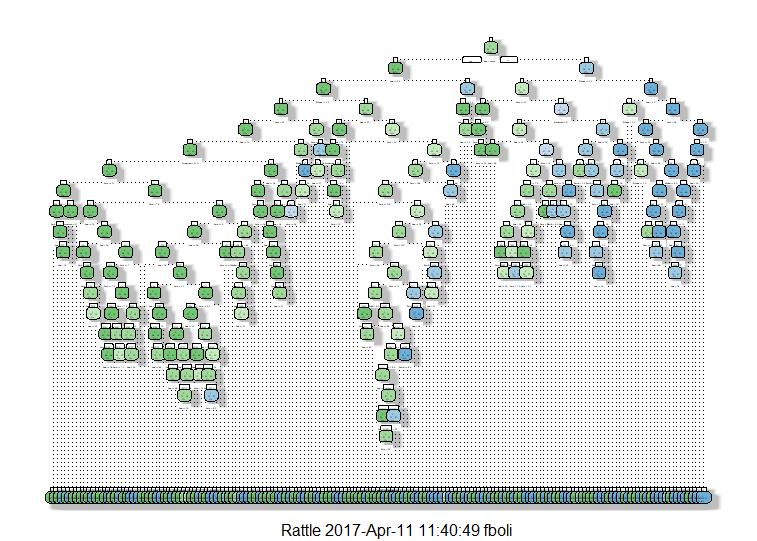
\includegraphics[width=14cm]{img/first-big-decision-tree}
	\caption{Primer árbol de decisión sin preprocesamiento dejando que llegue hasta el final}
	\label{fig:first-big-decision-tree}
\end{figure}

Que además de ser más ilegible obtiene una peor puntuación de 0.74163.

\subsubsection{Con preprocesamiento}

Una vez hemos realizado las tareas de preprocesamiento de la Sección \ref{sec:preprocesamiento}, podemos utilizar estas nuevas variables para aplicarlas al árbol de decisión:

\begin{lstlisting}[style=R]
fit <- rpart(Survived ~ Pclass + Sex + Age + SibSp + Parch + Fare + Embarked + Title + FamilySize + FamilyID,
             data=train, method="class")
\end{lstlisting}

Obteniendo el siguiente árbol:

\begin{figure}[H]
	\centering
	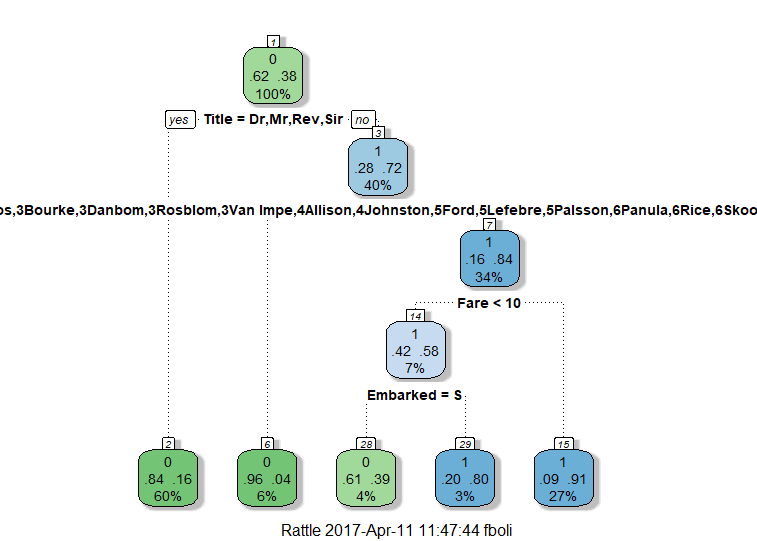
\includegraphics[width=14cm]{img/preprocessing-decision-tree}
	\caption{Árbol de decisión con preprocesamiento}
	\label{fig:preprocessing-decision-tree}
\end{figure}

Este árbol consigue mejorar la puntuación obteniendo la mejor puntuación personal hasta ahora de 0.79426.

\subsection{\textit{Random Forest}}

\subsubsection{\textit{Traditional Random Forest}}

Aunque casi hayamos alcanzado el 0.8 usando un árbol de decisión con preprocesamiento, el uso de \textit{random forest} puede mejorar.
\\ \\
Para utilizar el \textit{random forest} clásico hay que modificar la variable \texttt{FamilyID} que habíamos creado en la Sección \ref{sec:preprocesamiento} pues tiene demasiadas categorías. Para ello creamos una nueva reduciendo las categorías considerando familia pequeña con tres individuos o menos en vez de con dos:

\begin{lstlisting}[style=R]
combi$FamilyID2 <- combi$FamilyID
combi$FamilyID2 <- as.character(combi$FamilyID2)
combi$FamilyID2[combi$FamilySize <= 3] <- 'Small'
combi$FamilyID2 <- factor(combi$FamilyID2)
\end{lstlisting}

Y ya podemos aplicar el \textit{random forest}:

\begin{lstlisting}[style=R]
set.seed(14)
fit <- randomForest(as.factor(Survived) ~ Pclass + Sex + Age + SibSp + Parch + Fare + Embarked + Title
                    + FamilySize + FamilyID2, data=train, importance=TRUE, ntree=2000)
\end{lstlisting}

Con el que obtenemos una puntuación de 0.77033 más baja de lo esperado.

\subsubsection{\textit{Conditional Inference Random Forest}}

Viendo el inesperado resultado, vamos a probar una alternativa distinta al \textit{random forest} tradicional que a diferencia de éste permite usar variables con un número alto de categorías, por lo que podemos usar el \texttt{FamilyID} que no cuenta como pequeñas a las familias de tres miembros:

\begin{lstlisting}[style=R]
set.seed(14)
fit <- cforest(as.factor(Survived) ~ Pclass + Sex + Age + SibSp + Parch + Fare + Embarked + Title + FamilySize
               + FamilyID, data = train, controls=cforest_unbiased(ntree=2000, mtry=3)) 
\end{lstlisting}

Con el que obtenemos nuestra mejor puntuación de 0.81340

\subsection{\textit{XGBoost}}

En la literatura se presenta a \textit{XGBoost} como uno de los algoritmos más potentes y muchos ganadores de competiciones de Kaggle lo han usado. Por tanto, voy a intentar aplicarlo sobre los datos ya preprocesados:

\begin{lstlisting}[style=R]
param <- list(objective="binary:logistic", booster="gbtree", eval_metric="logloss")
nround  = 3382
set.seed(14)
clf <- xgboost(param =param, dtrain, nrounds=nround, min_child_weight=1,verbose=0)
pred <- predict(clf, dtest)
pred_final <- ifelse(pred>0.5,1,0) 
\end{lstlisting}

No obstante el resultado ha sido bastante peor al obtenido con el \textit{conditional inference random forest}, obteniendo 0.76077.

\section{Presentación y discusión de resultados}

Se han realizado distintas pruebas que se han ido presentando a lo largo de todo el documento.
\\ \\
Vimos como, tan solo dando como supervivientes a todas las mujeres y a los hombres como muertos se llegaba a tener una puntuación de 0.76555 y afinando un poco este pequeño árbol de decisión manual teniendo en cuenta la edad, la tarifa y la clase ya se sube hasta 0.77990.
\\ \\
No obstante, para hacer un árbol de decisión a mano, es mejor utilizar librerías de R que los hacen por ti y, sin ni siquiera realizar un preprocesamiento, logra mejorar a 0.78469.
\\ \\
Pero claro, los datos que tenemos no están preprocesados y, eliminando los valores perdidos de edad (usando regresión), embarque (usando la moda para dos valores perdidos) y tarifa (usando la mediana para el único valor perdidos) y agregando nuevos datos como el título (a partir del nombre) y la familia con el número de familiares y el apellido, podemos mejorar el resultado alcanzando el 0.79426.
\\ \\
Tras haber utilizado los árboles de decisión básicos se pasó a utilizar técnicas más potentes como \textit{random forest}, que en su versión de \textit{conditional inference} logra alcanzar una puntuación de 0.81340 (la más alta que he obtenido).
\\ \\
Por último se utilizó \textit{XGBoost} para intentar mejorar los resultados pero no se logró mejorar ya que los datos tienen mucho ruido pues dos personas con datos muy parecidos pudieron tener un desenlace distinto en cuanto a supervivencia.

\section{Conclusiones y trabajos futuros}

El \textit{dataset} de Titanic es uno de los más populares para empezar con la ciencia de datos. No obstante, obtener un resultado superior a 0.9 es muy complicado pues estamos ante un problema real donde dos personas muy parecidas pudieron tener un destino distinto.
\\ \\
Sin embargo, haciendo un análisis simple del problema se puede llegar a alcanzar el 0.77990 de acierto y utilizando técnicas como los árboles de decisión sobre los conjuntos de datos originales se llega al 0.78469. Y es que uno de los mayores saltos se encuentra aquí, cuando se preprocesan los datos antes de trabajar con ellos, pues el mismo algoritmo puede tener un punto de acierto más.
\\ \\
La técnica que mejor resultado me ha dado ha sido el \textit{conditional inference random forest} mejorando al \textit{XGBoost} que no funciona muy bien cuando hay ruido como el que se ha comentado.
\\ \\
Como trabajo futuro se podría intentar limpiar este ruido con técnicas como \textit{Smote} para volver a lanzar \textit{XGBoost} y ver si mejora los resultados de \textit{random forest}.

\section{Listado de soluciones}

\begin{table}[H]
	\centering
	\caption{Tabla de resultados}
	\label{tab:results}
	\begin{tabular}{|l|p{5.1cm}p{1.8cm}p{1.2cm}p{1.2cm}p{0.6cm}p{1.5cm}|}
		\hline
		\# & Descripción & Algoritmos y software empleado & Score (train) & Score (test) & Pos. & Fecha y hora \\ \hline \hline
		1  & Todas las mujeres sobreviven excepto aquellas que tengan Pclass=3 y Fare\textgreater=20. Todos los hombres mueren execpto aquellos que son niños y tienen Fare\textgreater=30 y PClass=1 o 2 & R & x & 0.77990 & 2629 & 4/11/17 9:00 \\ \hline
		2  & Todas las mujeres sobreviven, todos los hombres mueren & R & x & 0.76555 & 3806 & 4/11/17 9:05 \\ \hline
		3  & Árbol de decisión sin preprocesamiento & R (rpart) & x & 0.78469 & 2003 & 4/11/17 11:30 \\ \hline
		4  & Árbol de decisión sin preprocesamiento dejándolo crecer al máximo & R (rpart) & x & 0.74163 & 5484 & 4/11/17 11:35 \\ \hline
		5  & Árbol de decisión con preprocesamiento & R (rpart) & x & 0.79426 & 1250 & 4/11/17 11:40 \\ \hline
		6  & Traditional random forest con preprocesamiento & R (rpart, randomForest) & x & 0.77033 & 3479 & 4/11/17 12:45 \\ \hline
		7  & Conditional inference random forest con preprocesamiento & R (rpart, randomForest, party) & x & 0.81340 & 416 & 4/11/17 12:50 \\ \hline
		8  & XGBoost con preprocesamiento & R (rpart, kernlab, caret, xgboost) & x & 0.76077 & 4680 & 4/11/17 13:30 \\ \hline       
	\end{tabular}
\end{table}

%----------------------------------------------------------------------------------------
%	REFERENCIAS
%----------------------------------------------------------------------------------------

\newpage

\bibliography{referencias} %archivo referencias.bib que contiene las entradas 
\bibliographystyle{plain} % hay varias formas de citar

\end{document}